\documentclass[11pt]{article}

\usepackage[T1]{fontenc} % extended font encoding
\usepackage{enumerate} % lists
\renewcommand{\familydefault}{\sfdefault} % sans-serif
\usepackage{microtype} % better text justification
\usepackage{graphicx} % allow including pictures
\usepackage{color} % colors for pictures
\usepackage{xcolor}
\usepackage{lipsum}
\usepackage{pagecolor}
\usepackage{afterpage}
\usepackage[a4paper, landscape, margin=1.5cm]{geometry}
\usepackage{multicol}
\setlength{\columnsep}{1cm}
\fboxsep=5mm
\usepackage{blindtext}
\pagenumbering{gobble} % disable page numbering

\newenvironment{packed_enumerate}{
\begin{enumerate}
  \setlength{\itemsep}{1pt}
  \setlength{\parskip}{0pt}
  \setlength{\parsep}{0pt}
}{\end{enumerate}}

\newenvironment{packed_enumerate_i}{
\begin{enumerate}[I]
  \setlength{\itemsep}{1pt}
  \setlength{\parskip}{0pt}
  \setlength{\parsep}{0pt}
}{\end{enumerate}}

\pdfinfo{
   /Author (Zlosynth Instruments)
   /Title  (Kaseta - User Manual)
}

\begin{document}

\pagecolor{black}\afterpage{\nopagecolor}

\title{\textcolor{white}{MANUAL}}
\author{}
\date{}

% Left column
\begin{minipage}{0.4\textwidth}
\color{white}
\maketitle

% Overview
\noindent\colorbox{white}
{
\begin{minipage}{0.85\textwidth}\color{black}
What it is. Achordion allows you to do many things, but in essence, it is just a bunch of oscillators that never go out of tune or out of scale! Apart from playing anything between lush pads and hellish walls of sound, it enables you to easily jam with other musicians and explore characters of different scales.
\end{minipage}
}

\vspace{1cm}

% Specs
\begin{minipage}{0.8\textwidth}\color{white}
\begin{tabular}{@{}rl@{}}
  Width & 20 HP \\
  Depth & 28 mm \\
  Power & +12 V (85 mA), -12 V (7 mA) \\
  Input impedance & 100 kΩ \\
  CV inputs & 16-bit, 2 kHz \\
  Gate output & 5 V \\
  Audio & 24-bit, 48 kHz
\end{tabular}
\end{minipage}

\vspace{1cm}

% Features
\begin{minipage}{0.8\textwidth}\color{white}
\begin{tabular}{@{}l}
  - Aluminium panel with high-quality anodized finish \\
  - Based around Electro-Smith's Daisy Patch SM platform \\
  - Saturation \\
  - Compression \\
  - Harsh overdrive \\
  - Feedback designer \\
  - Granular synthesis \\
  - Four free moving heads \\
  - Tone contol \\
  - Rewind/speed simulation
\end{tabular}
\end{minipage}

\end{minipage}%
% Right column
\begin{minipage}{0.6\textwidth}
\vspace{8mm}
\begin{center}
  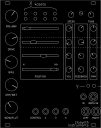
\includegraphics[width=1.0\textwidth]{schema.pdf}
\end{center}
\end{minipage}

\newpage
\color{black}



% Left column
\begin{minipage}[t]{0.35\textwidth}

\section {Warranty}

\lipsum[1]

\section{Installation}

Achordion is 20 HP wide. It is powered by a +12V/-12V 2x5 connector. The red stripe (-12V) must be connected on the side of the board marked with the white line. The module must be mounted in a Eurorack case.

\end{minipage}%
\begin{minipage}{0.05\textwidth}
\phantom{ }
\end{minipage}%
% Right column
\begin{minipage}[t]{0.55\textwidth}

\section{Controls, inputs and outputs}

Pre-amp
Tone
Saturation/drive
Bias
Wow
Flutter
Delay length
Head position
Head playback
Head feedback
Head pan

\end{minipage}

\newpage

\section{Pre-amp}

\section{Saturation}

\section{Delay}

Heads. Feedback vs blend. Ranges. Clock in. Gate out.

\section{Tone}

\section{Wow and flutter}

\section{Compression}

\section{Options}

Delay echo vs. audio rate
Quantization 1/8
Quantization 1/6
Wow cyclic vs. random
Flutter cyclic vs. random
Danger zone
Rewind/speed

\section{Configuration}

\section{Patch book}

* Basic hysteresis.
* Basic flutter with disabled hysteresis.
* Basic evenly spread one time delay.
* Basic feedback delay.
* Audio level delay. Just one slightly delayed head playing and feeding back.
  Perhaps on specific tones.
* Plain sine. All four heads playing in a small distance from each other.
  Producing reverb. Add flutter to make it forever moving and changing.
* Basic tremolo, just cyclic flutter.
* Custom wow/flutter using position modulation.
* Percussion rhythm.
* Delays comming back, with some heads close, some far to repeat way later.
* When bass drum and single oscillator tone play at the same time with high
  saturation and low bias, it works like sidechaining.
* Short cybmals, low bias cuts weak signal.
* Ping pong snare. Like Daughter's New Ways.
* Warm soft saturation on piano is nice.
* With non-warping delay, CV S and H input to delay value, selecting samples from
  the past.
* Playing a mellow song, slow speed. Fading when approaching end, switch to another head.

\section{Questions?}

\begin{center}
petr@zlosynth.com
\end{center}

\end{document}
